\documentclass[a4j,11pt,onecolumn,oneside,openany]{jsbook}
\usepackage[dvipdfmx]{graphicx}
\usepackage[dvipdfmx]{hyperref}
\usepackage{float}
\usepackage{amsmath}
\usepackage{amssymb}

\setlength{\textwidth}{\fullwidth}
\setlength{\evensidemargin}{\oddsidemargin}

\usepackage{atbegshi}
\ifnum 42146=\euc"A4A2 \AtBeginShipoutFirst{\special{pdf:tounicode EUC-UCS2}}\else
\AtBeginShipoutFirst{\special{pdf:tounicode 90ms-RKSJ-UCS2}}\fi

\title{効率とシステムサイズの関係に対する確率モデルによる考察}
\author{早稲田大学先進理工学部物理学科 4年\\
山崎研究室所属\\
藤本將太郎(1Y11A045-8)}
\voffset=-13mm
\hoffset=-8mm
\begin{document}
%\begin{titlepage}
\maketitle
\thispagestyle{empty}
%\end{titlepage}
\newpage
\section*{概要}
この論文では,系のサイズが変化するとその中の状態が変化する系,その中でも特に系のサイズが大きくなると個々の効率が減少するような系の解析のため,具体的なイメージとして会議を元にして確率モデルを作成し,それぞれのモデルに見られた性質を解析的に,あるいは数値シミュレーションによって解析した。その結果,境界条件やモデルの次元に強く依存した関係が現れることが確認され,有限のシステムサイズでピークをもつようなモデルも考えられた。

\newpage
\pagenumbering{roman}
\tableofcontents
\newpage
\pagenumbering{arabic}
\chapter{導入}

私達は普段の身近な生活の中で,サイズが変わるとその中の質や状態が変わってしまうと感じるものを見つけることができる。
それは会話とその人数の間の関係にもあるかもしれないし,共同作業を行うときのチームメンバーの人数かもしれない(\cite{kaigi4})。企業の大きさとその中の人間の従事度も異なるかもしれない。会議にやたら多くの人が参加していても,ほとんどの人はその会議を無意味なものだと見なすことになるだろう。世の中のおよそほとんどのスポーツやゲームなどは,参加する人数が予め決められていることが多い。よく練られたものであれば,この決められた人数より多くても少なくても,本来の楽しみを得ることはできないだろう。麻雀は4人でするから楽しめるのであり,会議は100人ではなかなか進まないものである。

このような現象は大変身近であり,私達にとって実感をもって受け入れられることなので,ほとんどの場合不文律にこの法則は受け入れられていると言っても良いだろう。

一方で相乗効果という点に着目すれば,一人で何かするよりも多くの人を交えて行ったほうが効率が上がるといった事例も多く存在していることだろう。しかしながら,この場合に関しても、多すぎることはまた別の問題を産むことがリ,多すぎることによって却って効率が下がるという事例も多く存在する。
こういったことを私達は無自覚の内に理解しているので,何かを大人数で共同して行う必要のあるときには,それをさらにいくつかのグループ,班,部署,といったより小さい単位に分割する必要を感じる。また,どれほどの人数で最小の組織を構成するのがよいか,ということは昔から考えられてきたことであり,最適人数に関する調査・研究が行われたり,詳細な研究はなされていなくとも各分野での情報が蓄積されたりしている。例えば教育の分野などではグループ学習や少人数授業の有効性が議論されることも多い。

さて,これまでに述べたような系のシステムサイズとその効率の間の関係は,何も人間を要素とした系でなくとも考えることができる。例えば,動物の体重と代謝率の間の関係も,同じ現象であるとみなすことができるかもしれない。動物学等の分野で知られている法則として,体重とその他の観測量の間の関係としてアロメトリー則と呼ばれるものがある。その一つが体重と代謝率の間の関係であり,特にこの関係のことをKleiber則と呼ぶ。これは様々なスケールの対象について調べられていて,代謝率$E$と体重$M$の間の関係は$E\sim M^{b}$のようにスケールされる。この指数については,データの取り方などによって異なるため,いくつか説があり,指数の大きさは$2/3$とする意見と$3/4$とする意見とがあり,また両辺の対数を取った関係式で右辺の$\log M$の2乗の項を考慮すればよりよくフィッティングできる,といったものもある。ここで重要視したいのは,指数の大きさがどちらか,ということではなく,その指数は1よりも小さい値をとる,ということである。これまで挙げてきたシステムサイズと効率の関係についてと同じように議論する余地があることが分かる。

この指数が生物種や成長過程における細胞組成の変化が本質的ではなく,その時点でのシステムのサイズが影響していることの一つの例として,ホヤの群体サイズと代謝率の間の関係も,同様に1乗より小さい指数でスケールされることが確かめられている。このホヤは無性生殖によって自分と全く同じ個体を増やして群体を形成し,群体同士のつながりはネットワーク上に張り巡らされた血管のつながりである。この群体の構成個数は実験者が物理的に切り離すことによって容易に変更でき,それによってサイズごとの代謝率を調べることができる。さらに,このホヤにはある時間周期ごとに一斉に分裂・増殖を行う"takeover"と呼ばれる現象が見られ,このときすべての個体間の血管つながりが切れ,このときの代謝率は同じ個体数の群体の代謝率よりも大きくなることが示されている。二つ目の例の場合は,これから増殖を行うために代謝率が増加したのだと見ることもできるのであるが,一つ目のサイズと代謝率の間の関係は,そのように簡単に説明されるものではない。これまでのKleiber則の説明としては,体温の維持と表面積との関係から2/3を導くものや,血管構造が大動脈から毛細血管に至るまでがフラクタル的であることに着目し,血液の流速と代謝率の間の関係を仮定して3/4を導くものがあった。しかしはじめの理論では変温動物や単細胞においてもこの関係が成り立つことのうまい説明ができない。また,二つ目の理論についても,より物理的な描像なため説得力はあるが,ホヤの場合,血管構造,特に血管の太さや長さに関して自己相似的とは言えず,また,その理論の中で仮定される"巨視的プールから微視的構造に向かう流れ"というものも見られないため,この理論では説明することはできない。したがって,引用元の記事の中では一つの仮説として以下のようなものが提唱されている。

\begin{quote}
『べき乗のサイズ効果は個体同士の局所的な相互作用によって生じ,takeover中には個体間の連絡が切れるため,サイズ効果が見られなくなる。同じユニットが局所的な相互作用をもつ系は,自己組織化臨界状態にある可能性があり,臨界状態とは相互作用に効果がべき関数で記載されるものである。ホヤを含め,動物は自己組織化臨界状態にあるのではないか。』
\end{quote}

ここまで述べて来たような,人間の作るシステムの中での最適人数の議論や,生物のアロメトリー則などは,統一した一つの理論として書ける可能性がある。このとき,それまで各モデルの中で重要だと思われてきた要素は,統一された理論の中でのある物理量に対応させることによって,どのモデルでも同じように書けるかもしれない。こうしたことを考えていくうちに,より抽象的にこの問題を考えることには何か意義があるのではという思いを抱くようになった。

この論文では,具体的なイメージとしては例の中で挙げられた会議を題材に議論を進めることにした。会議の進行プロセスを元に確率モデルを作成し,その解析を行って,その結果をまとめた。

\chapter{モデルの説明}

まずはじめに、作成した確率モデルに関しての説明と、その際追加で説明が必要と思われた場合にはその背景についても述べていくことにする。

会議について考える上で、システムサイズは会議に参加する人の人数であるとする。したがって、これから考えていくべき関係はこの人数と会議の"質"、成果との間の関係である。しかしながら、この"質"がどういった量として測れるのかは現段階で不明であるため、モデルを立てた際に得られる一般的な物理量から、質にあたるものを予測していく、というアプローチを取ることにする。

一口に会議と言っても世の中には様々な種類の会議が存在する。会社やグループの中で行われる会議の中には、すべての部署が一同に会し、その中でそれぞれの進捗状況など、情報を共有するための報告会議や、企画のためのアイデア出しなど、何か与えられた議題に沿ってそれぞれが自由に発言するタイプの会議もある。また、既に決定している内容に関して、それに関連のある人を集めて一度に口頭で説明するタイプの報告会も、一般には会議と呼ばれている。また、会議の進行方法もいくつかあり、会話と同じようにそれぞれの人が思い思いに発言する場合や、ファシリテーターと呼ばれる進行役が質問によってそれぞれの人の意見を引き出したり、意見をまとめたりして、会議の流れをコントロールする場合もある。このモデルで扱うのは、アイデア出しのようにそれぞれが自由に発言し、その意見がつながることによってよりよい案を得ることができる、という種類の会議であり、ファシリテーターのように全体の流れをコントロールできる独立した存在はいないものとする。

以上のような設定を考えた上で、これを確率論として扱うために、会議の中の言葉を抽象的なモデルで表すことにする。まず、「意見」とはまだ会議の中で発言されていない、それぞれの人がもつ考えをあらわすこととする。すべての意見が$a$個の異なる要素に分解でき、それぞれの要素は1つの実数値をもっているとすると、ある一つの意見$x$というのは、$\Omega \subset \mathbb{R}^{a}$上の一つの元
\[x = (x_{1}, x_{2}, \cdots ,x_{a}) \in \Omega\]
とすることができる。
\begin{figure}[H]
    \begin{center}
        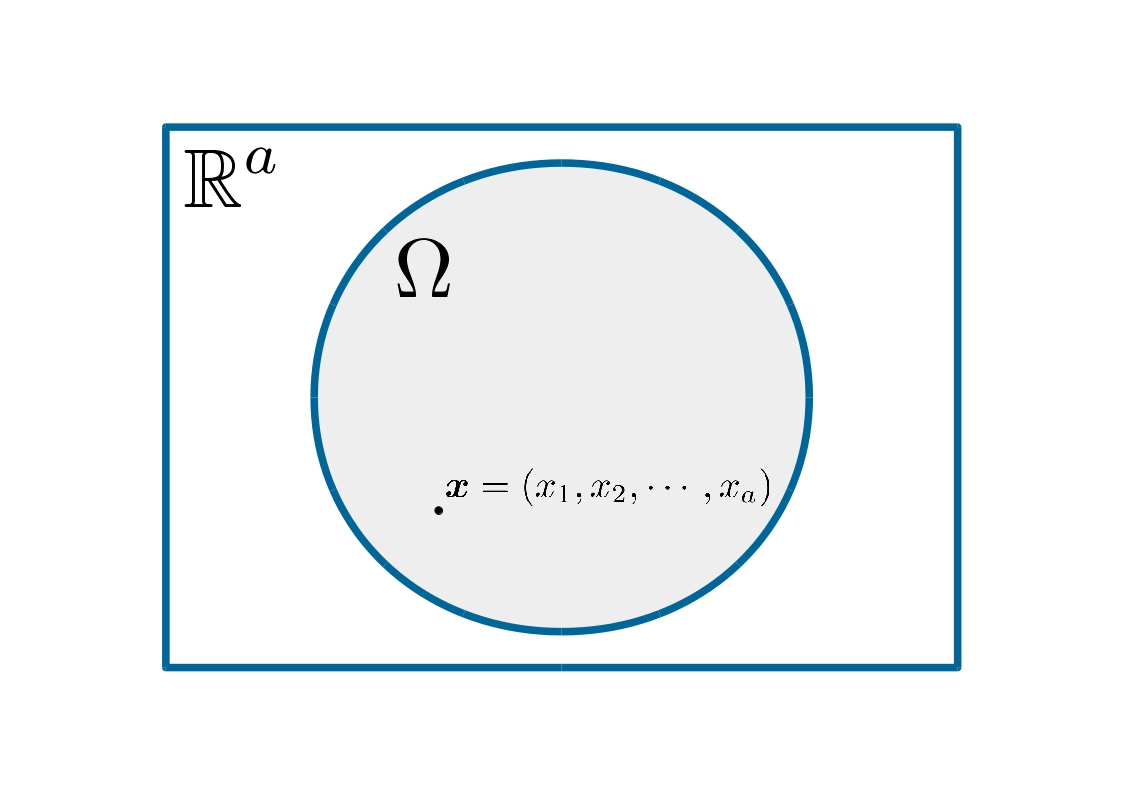
\includegraphics[width=12.5cm]{../img/ideaspace.jpg}
        \caption{$\mathbb{R}^{a}$上の空間$\Omega$と、その元である点$x$}
        \label{fig:f1}
    \end{center}
\end{figure}

また、この意見間の距離を定義すればこれらの点を元とする距離空間を定義することができる。距離の入れ方としてはユークリッド距離
\[d(x, y) = \sqrt{(x_{1} - y_{1})^{2} + \cdots + (x_{a} - y_{a})^{2}}\]
を考えることとする。

次に、「参加者」について考える。参加者は会議の中で自分の中にある意見を発言していくのであり、参加者それ自体は意見の集まりである。すなわち意見空間$\Omega$上の部分空間$X_{i}$が参加者$i$を表すとする。$x_{ik}$が人$i$のラベル$k$の意見であるとすると、人$i$が$s_{i}$個の意見を持っているとき、
\[X_{i} = \{x_{i0}, x_{i1}, \cdots , x_{is_{i}}\}.\]
一般に
\[X_{i}\cap X_{j} = \emptyset\ \ \  \text{when}\ \ \ i \neq j\]
である必然性はないが、このモデルでは上式を採用することとする。したがってモデルの中で扱う意見空間$\Omega_{0}$は、参加者が$N$人集まったとき、$X_{i}$の直和集合
\begin{align}\Omega_{0} &= \bigcup_{i = 1}^{N} X_{i} \nonumber \\
&= \sum_{i=1}^{N} X_{i} \end{align}
となる。

モデルの作成に際し、会議の進行に関していくつかの仮定をおいて考えていくことにする。これらの仮定が本質的であるような場合にはまた別のモデル化を考える必要があるが、ひとまず以下の仮定を受け入れることにして、その上でモデルを作成することにした。

仮定:
\begin{itemize}
    \item 一度に発言できる人は一人まで
    \item 一人当たりの発言時間は参加人数に依らない
\end{itemize}

このように仮定すると、会議という過程を、1つの時間発展するネットワークの生成過程であると見なすことができる。すなわちある参加者に必ず属する点をルールにしたがって各時刻ごとに選択していき、その時意見間の間にも与えられた別のルールによってエッジを結んでいくとする。このようにすると、終了時刻$K$が経過した時には、意見間のネットワークと、参加者間のネットワークを得ることができる。このネットワークの特性の中に、会議の質となりうる量があるとして、この描像のもとに意見$x$や参加者$X_{i}$の選択に関してのルールを与えていくことにする。

以降の議論では、特に必要のない限り、上で定めた記号と言葉を使い、「会議、意見、参加者」といった言葉は使わないことにする。

点$x$の選び方としては、
\begin{enumerate}
    \item 集合$X_{i}$を選び、その中から$x$を選ぶ方法
    \item 点$x$を選び、その点の情報から、$X_{i}$を決める方法
\end{enumerate}
の二つがある。

それぞれの場合について、$x$と$X$を選ぶ確率が互いに独立な場合と、そうでない場合にさらに分けて考えることができる。

したがって、考えるべきは
\begin{itemize}
    \item $X_{i}$の独立な選び方
    \item $x$の独立な選び方
    \item $X_{i}$が選ばれたときの$x$の選び方
    \item $x$が選ばれたときの$X_{i}$の選び方
\end{itemize}
の4つである。

\chapter{各モデルにおける結果と考察}

この章では,2章で設定したモデル化の方法を用いて,$x$と$X_{i}$の選択に関するルールと,$x$間のエッジの結び方に関するルールを定め,そのルールに従ったときにはどのようなネットワークの特徴量が得られるかについて,それぞれ見ていくことにする。3.1節では$X_{i}$を等確率で選び,その中から$x$が一様に選ばれる場合,3.2節では$X_{i}$を一つ前の$X_{j}$によって決まる確率で選び,その中から$x$が一様に選ばれる場合を考える。3.3節では,$X_{i}$に依らず過去の点$x$を参照にして次の点を選択する場合を考察し,3.4節では3.3節の場合を拡張し,近距離にある点をクラスター化し,そのクラスタ―$y$同士のネットワークを考えたモデルを考察する。それぞれの場合について,解析的に計算ができるところは計算によって理論値を求め,シミュレーションの結果と対応するかを確かめた。また,それぞれの場合について,特にシステムサイズ$N$とどう関連するのかに重点をおいて考察を行った。

\section{$X_{i}$を等確率で選び,その中から$x$が一様に選ばれる場合}

この設定は,はじめに$N$個の集合$X$から1つの$X_{i}$選択し,点$x$はそれぞれの $X_{i}$について$\Omega = [0,1]$に一様に分布しているとする。
このとき,$X_{i}$の数$N$が変化しても,$x$についての選び方は同じであるから,$x$の作るネットワークだけでは,本来考えたい$N$との間の関係は見ることができない。
しかしながら,選ばれた点のネットワークに関する性質を調べるには良い練習となる。

$X_{i}$から$k$番目に点が選ばれ,その後時刻$k+1$に$X_{j}$から点が選ばれる確率は,$X_{i}$の数$N$として
\[p_{i}(k,j) = p(N) = \frac{1}{N}\]
のように,直前の履歴に依存せず,等確率である場合を考えている。

このとき,$x$は$[0,1]$の間の値を一様な確率で取るとしていたので,そうして得られた確率変数$x$に関して,
確率密度関数$f(x)$は
\[f(x) = 1\ \ \ (0\le x \le 1)\ \ \ \text{otherwise}\ \ 0\]
であり,累積分布関数$F(x)$は
\[F(x) = x\ \ \ (0\le x \le 1)\]
である。

時間発展によって点が選ばれていくごとに,その点と距離$r$より近い位置にある点との間にすべてエッジを張っていくことにする。
すなわち,この問題はある閾値$r(0<r\le1)$を定めた時に,時刻$k$で選ばれた点$x_{k}$を中心とする領域$[x^{k}-r, x^{k}+r]$の中に入るそれまでに出た点の数はいくつか,という問題に帰着される。

すなわち図\ref{fig:f2}のような状況を考えていることになる。
\begin{figure}[H]
    \begin{center}
        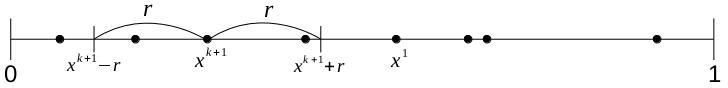
\includegraphics[width=10cm]{../simple1/simple001_1.jpg}
        \caption{$[0,1]$の数直線上で閾値$r$で定められる領域}
        \label{fig:f2}
    \end{center}
\end{figure}
一様な確率で$[0,1]$の間の数が選ばれるとき,その確率変数が$[\max(0,x-r), \min(x+r,1)]$の範囲に入っている確率は,確率密度関数を用いて,
\begin{align}
p(\max(0, x-r), \min(x+r, 1)) &= \int ^{\min(x+r,1)}_{\max(0, x-r)} 1 dx \nonumber \\
&= \left[ x\right]^{\min(x+r,1)}_{\max(0, x-r)}
\end{align}
よって
\begin{eqnarray}
p(x,r)= \left\{ \begin{array}{ll}x+r & 0\le x< \min(r,1-r) \nonumber \\
p(r) = \min(2r, 1) & \min(r, 1-r)\le x \le \max(1-r, r) \nonumber \\
1 - x+r & \max(1-r, r) < x \le 1
\end{array}\right.
\end{eqnarray}
を得る。

これはグラフにすると,図\ref{fig:f3}のようになる。
\begin{figure}[H]
    \begin{center}
        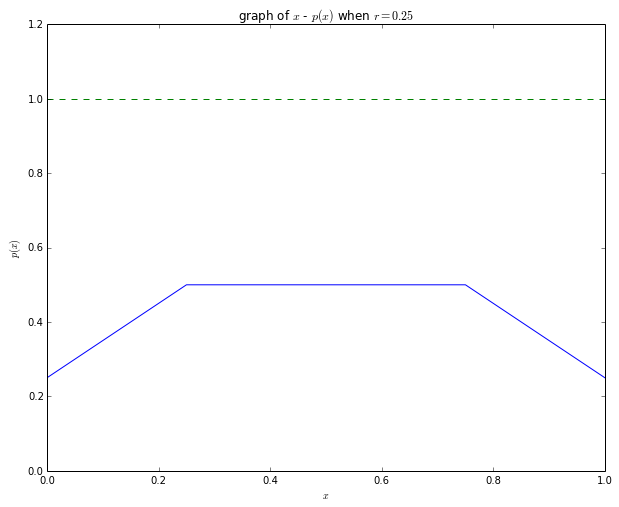
\includegraphics[width=10cm]{../img/fig3.png}
        \caption{$r=0.25$のとき,それぞれの位置$x$において他の点を1つ見出す確率$p(x)$}
        \label{fig:f3}
    \end{center}
\end{figure}

$k+1$番目に点$x_{k+1}$が選ばれたとき,$k$番目までに選ばれた点のうち$y$個の点が領域$[\max(0,x-r), \min(x+r,1)]$の中に存在する確率は,
\begin{eqnarray}
_{k}C_{y}p(r)^{y}p(r)^{k-y}
\label{eq:e1}
\end{eqnarray}
で表せる。
ここで注意すべき点は,$p(x_{k}, r)$は$x_{k}$によって変わるものであったから,$x$に対して期待値を取ったものを考えなければならないことである。
$p(r)$はそのようにして得られた期待値であることを意味している。

$p(r)$を求めると,
$0<r\le0.5$のとき
\begin{align}p(r) = E(p(x, r)) &= \int^{r}_{0}x+r\mathrm{d}x + \int^{1-r}_{r}2r \mathrm{d}x + \int^{1}_{1-r} 1-x+r \mathrm{d}x\nonumber \\
&= \left[\frac{x^{2}}{2} + rx \right]^{r}_{0} + \left[ 2rx\right]^{1-r}_{r}+ \left[ x-\frac{x^{2}}{2} + rx\right]^{1}_{1-r}\nonumber \\
&= -r^{2} + 2r \end{align}
$0.5<r\le1$のときも同様にして
\[p(r) = E(p(x,r)) = -r^{2} + 2r\]
である。

また,式(\ref{eq:e1})は
\[P[X=y] =\ _{k}C_{y}p(r)^{y}(1-p(r))^{k-y}\]
のように書けば明らかなように,確率変数$X$に対するパラメータ$k,p$の二項分布$B(k,p)$を表している。

この時,確率変数$X$に対する期待値と分散は,
\[E(X) = kp(r)\]
\[V(X) = kp(r)(1-p(r))\]
である。

時刻$k$が大きい時,具体的には
\[kp(r) > 5,\]
\[kp(r)(1-p(r)) > 5\]
をみたす$k$のとき,二項分布は正規分布に近似できるので,期待値は中央値とほぼ等しくなる。
すなわち,$y=kp(r)$より多くの点を見出す確率$P[X\le y]$は,どんな時刻$k$においても$1/2$となる。

すなわち,時刻の依存性はないため,$x_{k+1}$のまわりの領域に$y$個以上の他の点が存在する場合を1,存在しない場合を0とすれば,これらの起こる確率は,それぞれ$1/2$であり,$k$回目に$y$個以上のエッジが張られる確率は,$p=1/2$の幾何分布に従う:
\[P[X=k] = \left( \frac{1}{2} \right)^{k}\]
このときの期待値と分散は
\[E(X) = \frac{1}{p} = 2\]
\[V(X) = \frac{1-p}{p^{2}} = 2\]

すなわち,これまでのような場合を考えたとすると,平均として2回で$y$個以上のエッジが張られ,ほとんどの試行は$1\sim3$回でその値に到達することが分かる。
しかし,これは先程述べたような二項分布の正規分布への近似ができない領域であることに注意が必要である。

\subsection{$X_{i}$を一つ前の$X_{j}$によって決まる確率で選び、その中から点$x$が一様に選ばれる場合}

次に考えるのは、$X_{i}$の選び方が、一つ前の$X$による確率で決定するような場合である。この確率を定めるにあたり、会議として自然と思われる$X_{i}$間に距離が定義でき、その距離にしたがって確率が決まるような問題を考えることとした。このとき距離の計算に用いることができるパラメータの数を$b$とし、距離として$b$次元ユークリッド距離を考えることにする。

すなわち$b$個のパラメータを要素とする元からなる空間$X$があったとき、

距離関数$d: X \times X \rightarrow \mathbb{R}$が

$$d(x, y) = \sqrt{\sum_{i=1}^{b}(x_{i}-y_{i})^{2}}\ \ ,\ x,y\in X$$

と書けることを意味する。実際の場合には、各データ同士の相関を考慮に入れたマハラノビス距離などのほうが適当な場合もあるかもしれないが、まずはイメージしやすいということでユークリッド距離を考えた。

以下では、記述を簡単にするため、$X_{i}$と$X_{j}$の間の距離を$d_{ij}$と書くことにする。

時刻$k$に$X_{i}$が選ばれ、その後時刻$k+1$に$X_{j}$から点$x_{k+1}^{j}$が選ばれる確率$p_{k}(i,j)$は、距離$d_{ij}$の関数として、次のようにできる。

$$p_{k}(i,j) = \frac{g_{k}(d_{ij})}{\sum_{j} g_{k}(d_{ij})}$$

ここでの関数$g$の選び方によって、距離の大きさがどのように確率に重みを持たせるかということが決定される。一般に$g$は時刻$k$によって変化してもいいので、添字$k$をつけて時刻$k$における関数であることを表した。

単純な例として$g_{k}(d) = const.,\ ^{\forall}k, d\in \mathbb{R}^{1}$とすると、距離に依らず$X_{i}$が選ばれるわけなので、3.1節の$X_{i}$の選び方と同じである。

$g(d)$は$[0, +\infty]$で定義される非負の実関数であればよい。

ex)

$$g(d) = \frac{1}{d+1}$$

$$g(d) = e^{-d}$$

$$g(d) = \left\{ \begin{array}{ll} c & (0\le d \le 1/c) \\
1/d & (d>1/c) \\
\end{array}\right., \ \ c>0$$

しかし、ここで注意すべき点として、どの$X_{i}$が選ばれたとしても、3.1で考えたように、どの$X_{i}$も$[0,1]$から一様に点$x$を取るから、結局点$x$について見たときの試行は同様のことをしており、どの$X_{i}$が選ばれるかは本質的な問題にはならないことが分かる。

これまでの設定を用いて数値シミュレーションを行った結果を図\ref{fig:f4}$\sim$\ref{fig:f6}に示す。シミュレーションでは、確率を決める距離の関数$g(d)$として
$$g(d) = e^{-d}$$
を採用し、$x$の次元$a=2$、$X_{i}$の数$N=6$と設定した。

図\ref{fig:f4}の中の青い丸が$X_{i}$の位置を表しており、それぞれの丸の大きさは、一回の試行において選択された頻度を表したものとなっている。円の間に張られた線分とそこに記された数字の組は、1番目の数字をラベルとしてもつ$X_{i}$のあとに2番目の数字をラベルとしてもつ$X_{j}$が選ばれたことを意味している。
図\ref{fig:f5}で青色の曲線で表されているのは、時刻$k$に選ばれた点$x$のまわりの$r$で決まる領域の中に入った、それまでに選択された点の数である。また、このグラフで緑色の直線として表されているものは、3.1のように計算で求めた値であり、
$$l = (-r^{2} + 2r)k$$
であった。同じようにして偏差についても計算ができており、
$V(l) = \sqrt{(-r^{2} + 2r)(1+r^{2}-2r)k}$
である。これはグラフにおいて緑色の領域として描かれている。
図\ref{fig:f6}は、時刻$k$までに張られたエッジの数の総和を表しており、この中の緑色の曲線も、計算で求めることのできるものであった。
$$L = \frac{1}{2}(-r^{2} + 2r)k^{2}$$


\begin{figure}[H]
    \begin{center}
        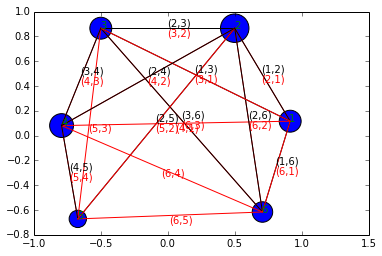
\includegraphics[width=12.5cm]{../download2_2.png}
        \caption{$X_{i}$の選択された頻度と$X_{i}$間ネットワーク}
        \label{fig:f4}
    \end{center}
\end{figure}
\begin{figure}[H]
    \begin{center}
        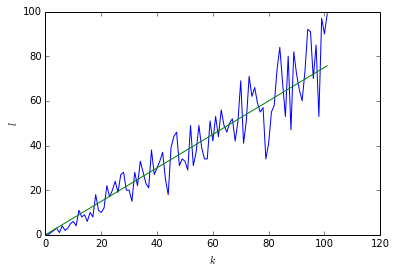
\includegraphics[width=12.5cm]{../download2_3.png}
        \caption{時刻$k$とその時張られたエッジの本数$l$との間の関係}
        \label{fig:f5}
    \end{center}
\end{figure}
\begin{figure}[H]
    \begin{center}
        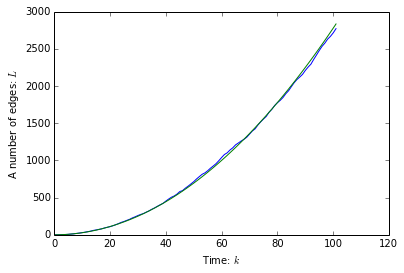
\includegraphics[width=12.5cm]{../download2_4.png}
        \caption{時刻$k$までに張られたエッジの数の総和$L$}
        \label{fig:f6}
    \end{center}
\end{figure}



\section{過去の点$x$を参照にして次の点を選択する場合}

1の場合には、$X_{i}$を選ぶ確率とそのうえで$x$が選ばれる確率は独立であるというものであった。しかし、これまで考えたように、単にそのようなモデルを考えただけだと$X_{i}$の数$N$の効果をうまく反映できないように思える。したがって、次に考えるモデルは前に選ばれた点に近い点が選ばれることにし、そのときその点をもつ$X_{i}$が選ばれたとするモデルである。

$X_{i}$はそれぞれ$s_{i}$個の点をもっており、モデルの設定時に仮定したとおり、これらの点は異なる$X$同士で共有されることはない。はじめに点$x_{0}$が与えられ、次に時刻$1$では、それぞれの$X$の中で最もその点に近いものを選び、より近いものをもった$X$の順に整列する。この$X$の順番にしたがって、$X_{i}$にそれぞれに割り当てられた確率$P_{i}$で、実際にその点$x$が選択されるかどうかが決定する。点が選択されない場合(確率$1-P_{i}$)ときは、$X$の順番で次の順番になっているものについて、同様の試行を繰り返す。もしすべての$X$について点$x$が選択されないときは、時刻$k$を一つすすめ、その時刻には$x_{0}$が選ばれたとする。
\begin{figure}[H]
    \begin{center}
        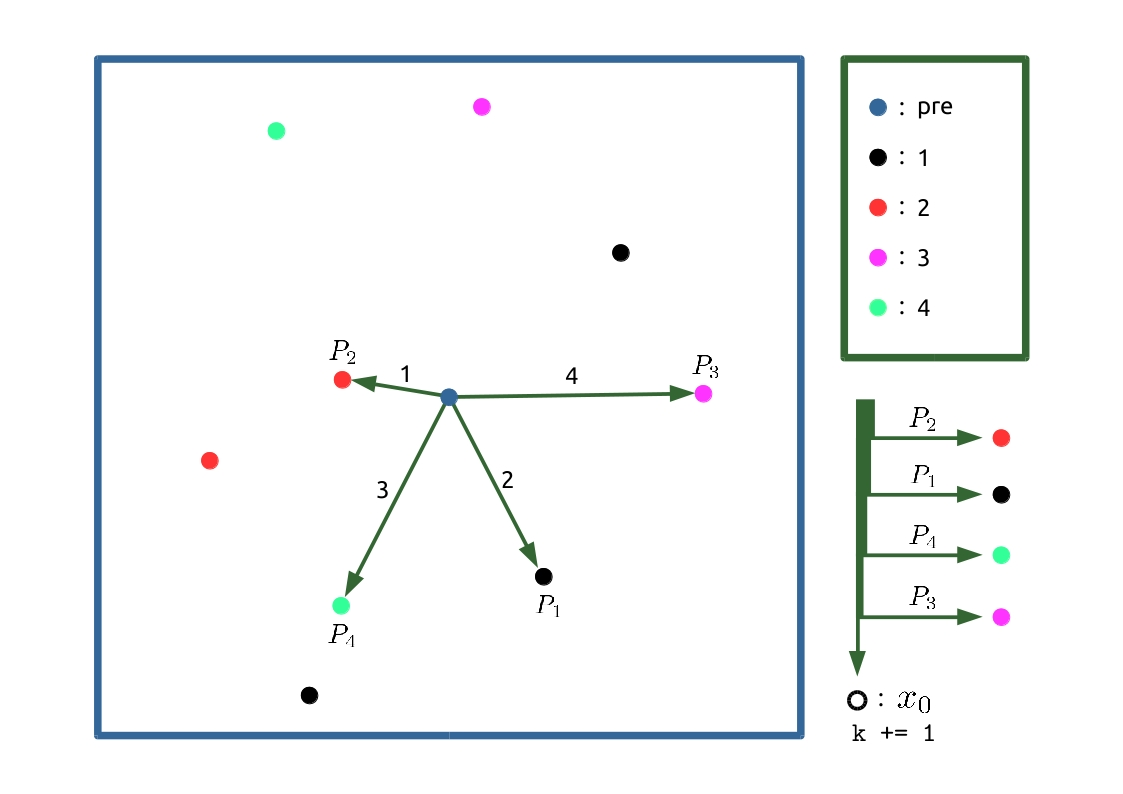
\includegraphics[width=12.5cm]{../img/figure2.jpg}
        \caption{$[0,1]$の数直線上で閾値$r$で定められる領域}
        \label{fig:f8}
    \end{center}
\end{figure}

図\ref{fig:f8}を用いて説明する。中心にある"pre"と名のついた点が参照する一つの点であり、この次の時刻に選ばれる点の選び方は、まずそれぞれの$X_{i}$について"pre"に最も近い点を選び、その近さの順に順番を付けることにする。図で青枠内の緑の矢印に示された数字がそれぞれの$X_{i}$の順番である。この順番にしたがってそれぞれの$X_{i}$に割り当てられた$P_{i}$にしたがって実際にその点が選ばれるかどうかが決まる。右下の矢印はそのことを表したフローチャートになっている。すべての$X_{i}$について点が選ばれなかった場合、時刻を一つ進め、はじめの点$x_{0}$を選択する。

参照する点の選び方として、以下のような場合分けを考えた。

\begin{enumerate}
    \item なし (case 1)
    \item 一つの点
    \begin{enumerate}
        \item 時刻0における点 (case 2)
        \item 一つ前の時刻の点 (case 3)
        \end{enumerate}
    \item 二つの点
    \begin{enumerate}
        \item 時刻0における点 + 一つ前の時刻の点 (case 4)
        \item 二つ前の時刻までの点 (case 5)
        \end{enumerate}
\end{enumerate}

\subsubsection{過去の点の影響を受けない場合 (case 1)}

$X_{i}$が$X$の配列の中で$r+1$($r = 1, 2, \cdots , n-1$)番目に選ばれたとき、$X_{i}$まで順番が回ってくる確率は
\[p_{r+1}(i) = \frac{\sum_{J = \langle j_{0}, \cdots ,j_{r-1} \rangle _{r}}\prod_{j\in J}(1-P_{j})}{_{n-1}C_{r}}.\]
ここで$J = \langle j_{0}, j_{1}, \cdots ,j_{r-1} \rangle_{r}$は、$i$を除く$n-1$個の要素から$r$個選んだときの組み合わせのうちの1揃いをあらわすことにする。

また、1番目に$x$を選択する権利を得たときに、選択権が回ってくる確率は当然
\[p_{1}(i) = 1\]
である。

説明のための具体的な例として、$N = 5, n = 5, i = 1, r = 2$とすると、$X_{1}$までに2つの$X$が選択権を得ているはずであり、その2つの組み合わせは$(0,2), (0,3), (0,4), (2,3), (2,4), (3,4)$の6つの組み合わせがある。上の式では$J$の一つは$(0, 2)$であり、このとき$j_{0} = 0, j_{1} = 2$である。この$J$に関して和をとり、組み合わせの数$\ _{4}C_{2} = 6$で割って期待値を求めている。
\begin{align}
p_{r+1}(1) &= \left[(1-P_{0})(1-P_{2}) + (1-P_{0})(1-P_{3}) + (1-P_{0})(1-P_{4}) \right. \nonumber \\
&\ \left. + (1-P_{2})(1-P_{3}) + (1-P_{2})(1-P_{4}) + (1-P_{3})(1-P_{4}) \right]/6
\end{align}
$X_{i}$が選択権の順番で$r$番目になる確率は等しいので、$r$に関する平均をとり、$P_{i}$をかければ、これは$X_{i}$から点が選ばれる確率の期待値となる。

\[p(i) = \frac{\sum_{r=0}^{n}p_{r}(i)P_{i}}{n}.\]

このとき得られた確率は$X_{i}$によって異なり、期待値としては毎時刻ごとにそれぞれの$X_{i}$がその確率が点が選択されることになり、単純な確率過程に帰着できる。


\subsubsection{1つ前の点を参照する場合}

それぞれの$X_{i}$が、配列の順番が回ってきたときに同じ確率$p$で点を選ぶとしたとき、はじめに与えられた点$x_{0}$のみを参照にしてその点からの近さのみで次の点を選ぶ場合と、一つ前の点のみを参照にして次の点を選ぶ場合の二つの場合に関してシミュレーションを行った。このとき、シミュレーション時に変更できるパラメータとしては、$X_{i}$の数$N$、$X{i}$あたりにもつ点の数$S$、順番が回ってきたときに点を選択する確率$p$がある。

点$x$と$y$の間の近さの指標として、$a$次元ユークリッド距離
\begin{align}D(x, y) &= d(x,y) \nonumber\\
&= \sqrt{(x_{1} - y_{1})^{2} + (x_{2} - y_{2})^{2} + \cdots + (x_{a} - y_{a})^{2}}\end{align}
を用いることにする。シミュレーションでは、描画の簡単さとイメージのしやすさから$a=2$の場合を考えることにした。

以下に作成したプログラムを用いて得られたネットワークの例を示す(図\ref{fig:f9}, 図\ref{fig:f10})。このとき、$K=30$, $N=6$, $S=30$, $p=0.6$としている。
図\ref{fig:f9}は、はじめに与えられた点$x_{0}$のみを参照にしたときに得られたネットワークのグラフであり、このとき、中心付近の青色の点は$x_{0}$であり、この点とつながっているエッジは薄い灰色で描画されている。それ以外の黒い線分は、選ばれた意見同士のエッジを表しており、ノードに振られた数字はその点が選ばれた時刻$k$を示している。
\begin{figure}[H]
    \begin{center}
        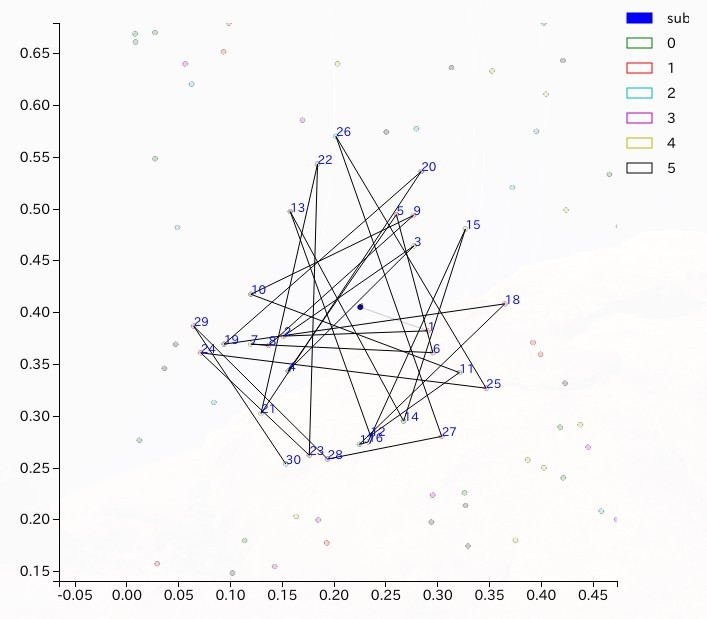
\includegraphics[width=10cm]{../simple3/case_2.jpg}
        \caption{$x_{0}$のみを参照にして次の点を選んだ場合のシミュレーション結果の一例}
        \label{fig:f9}
    \end{center}
\end{figure}
\begin{figure}[H]
    \begin{center}
        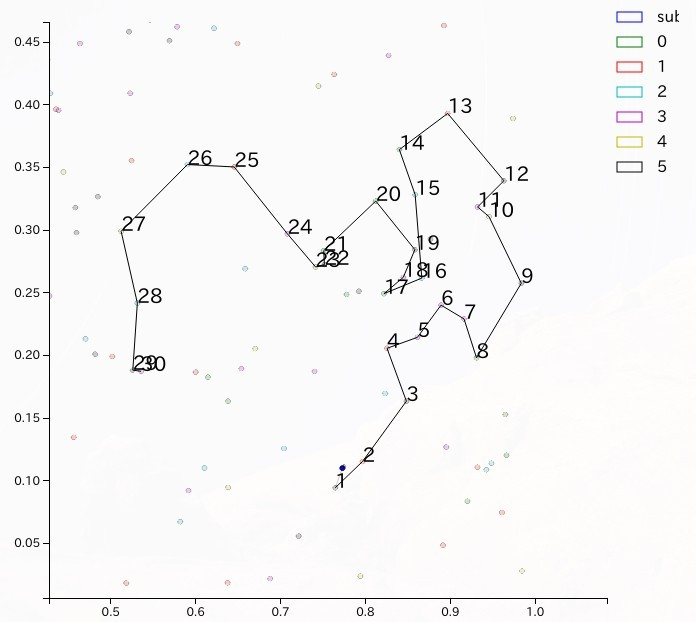
\includegraphics[width=10cm]{../simple3/case_3.jpg}
        \caption{1つの点のみを参照にして次の点を選んだ場合のシミュレーション結果の一例}
        \label{fig:f10}
    \end{center}
\end{figure}

\subsubsection{二つの点を参照して次の点を選択する場合}

次に、過去の二つの選択された点を参照して、その2点から近い位置にあるてんを次に選ばれる点の候補とする場合を考えることにする。このとき、2点からの近さの指標は、うまくこちらで決めてやる必要がある。近さの指標となる一つの例として、二つの点を焦点とした楕円を考えることができる。すなわち2つの点からの距離の和が等しい点はすべて同じ距離にあると見なすような近さが考えられる。したがって2点$(y, z)$からの点$x$の近さの指標$D(x, (y, z))$は、通常の$a$次元ユークリッド次元を$d(x,y)$と表すと、
$$D(x, (y, z)) = d(x,y) + d(x, z)$$
のように書けることになる。また、この考えが役に立つのは、それぞれの距離を足すときに適当な正の係数を掛けることによって、2つの点のどちらへの近さを優先するのかという条件を付け加えることができる点である。すなわち、正の定数$\alpha$ ,$\beta$を用いて、
$$D(x, (y, z)) = \alpha d(x,y) + \beta d(x, z)$$
のようにも書くことができる。参照する点をさらに増やしたい場合にも、それらの点との間の距離に係数を掛けて足せばよいので、いくらでも参照点を増やすことは可能である:
$$D(x_{k+1}, (x_{1}, x_{2}, \cdots , x_{k})) = \sum_{i=1}^{k}w_{i}d(x_{k+1}, x_{i})\ \ (w_{i} > 0)$$
また、別の近さの指標として、ベクトル$\vec{Y} = y-x$, $\vec{Z} = z-x$として
$$D(x, (y,z)) = |t\vec{Y} + (1-t)\vec{Z}|\ \ (0 \le t \le 1)$$
とする方法もある。このとき、右辺の括弧の内部が表すベクトルは、点$y$,$z$を結んだ線分$YZ$を$(1-t):1$に内分する点のベクトルを示しており、$D$はその点から$x$までのユークリッド距離を表すことになる。

シミュレーションでは、はじめに挙げた近さの指標を用いて選択権の順番を決定することにする、図\ref{fig:f11}と図\ref{fig:f12}は、それぞれ$x_{0}$の点と一つ前の点を参照にして点を選択する場合と、二つ前までの点を参照にして点を選択する場合のシミュレーションを行ったときに得られた結果の例である。

\begin{figure}[H]
    \begin{center}
        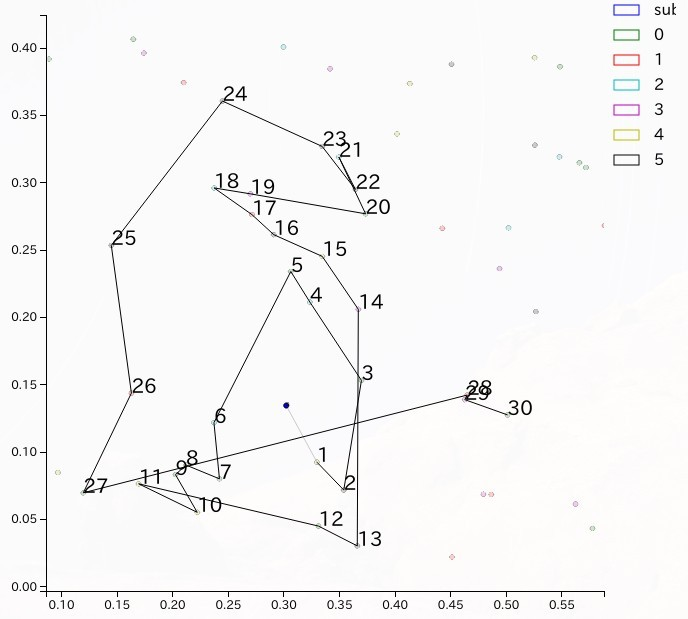
\includegraphics[width=10cm]{../simple3/case_4.jpg}
        \caption{$x_{0}$と一つ前の点を参照にして次の点を選んだ場合のシミュレーション結果の一例}
        \label{fig:f11}
    \end{center}
\end{figure}
\begin{figure}[H]
    \begin{center}
        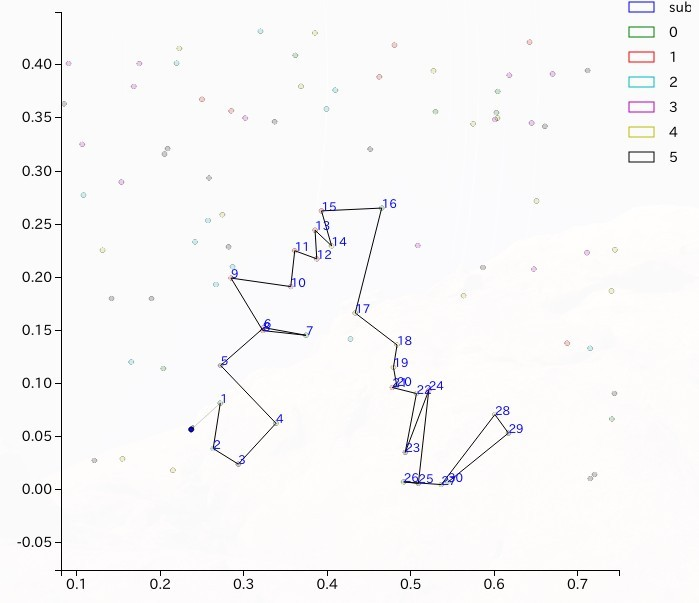
\includegraphics[width=10cm]{../simple3/case_5.jpg}
        \caption{二つ前までの点を参照にして次の点を選んだ場合のシミュレーション結果の一例}
        \label{fig:f12}
    \end{center}
\end{figure}

\section{近距離の点をクラスター化するモデル}

このモデルでは,3.2で考えたモデルと同様に,点$x$をそれまでに選択された点からの近さで選んでゆくようなモデルを考えることにする。

これまで考えてきたモデルとの大きな相違は,点を選択していく過程をは始める前に,すべての$x$について,自分から近い位置にある点同士をエッジで結んでいき,クラスターを形成することである。こうして得られたクラスター$y$について,その一つ前に選ばれた点$x$から最も近い点を含む$y$から,次の時刻の点が選ばれるとする。このとき$y$の中から点を選ぶ方法は,そのクラスター内に含まれる点の属するそれぞれの$X$に割り当てられた重みによって決定されるとする。

このモデルの着想を得るにあたって,実際の話し合いの際に,人が多くなることによって人がどのように考えるか,ということに影響を受けている。すなわち,話し合いに参加する人が多いほど,自分の意見と同じ様な意見をもつ人がいるだろう,と思う効果であり,$X_{i}$に割り当てられた重みは,個人の発言力をあらわしていると考えることができる。

シミュレーションにおいてクラスター化を行う際には,自分と他の点との間の距離を測り,これが$r$より小さいものの間にエッジを張ることにする。このとき,(特に$r$が小さいときに)効率よく近傍点を探すことができるよう,はじめに全体を長さ$l(>r)$の正方形の領域(セル)に分割し,それぞれの点がどのセルに属しているかを記録しておく。このようにすると,近傍点を探す際には,自分の属するセルとその周囲8マスを含めた9つのセルの中にある点のみについて調べればよい。このようにしてすべての点について順番に閾値$r$の内部にある点を選択していく。このとき領域内に入ったすべての点にクラスター番号が与えられていない時には,通し番号でクラスター番号を割り当てる。閾値$r$で定められる領域内に,より小さいクラスター番号をもつ点が存在する時には,その中で一番小さいクラスター番号を,接続しているすべての点に同じクラスター番号を付与する。このようにすれば,既に存在するクラスターとの間の融合などを考慮に入れたクラスター化が行える。また,今回のシミュレーションでは,$X_{i}$の違いによる選択確率の違いはないものとした。

図\ref{fig:f15}に,$r=0.07, K=20, N=4, S=20$としたときに実際にどのようにクラスターが形成され,点が選択されていくかの様子を示した図を載せる。グラフで薄いグレーで描かれた線はノード間の距離が$r$より小さいために張られたエッジであり,これが連結しているひとまとまりがクラスターである。青色の線は,選ばれた点同士をつなぐ(有向)エッジであり,振られている番号は時刻$k$に張られたエッジであることを表す。
\begin{figure}[H]
    \begin{center}
        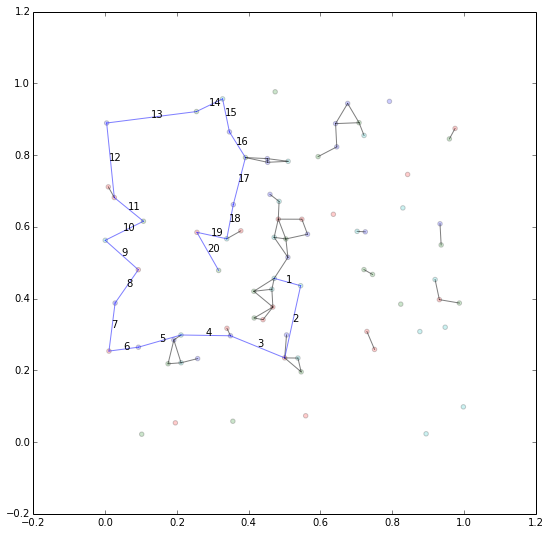
\includegraphics[width=10cm]{../img/cluster.png}
        \caption{近傍点をクラスター化するモデルのシミュレーション結果の例}
        \label{fig:f15}
    \end{center}
\end{figure}

このシミュレーションでは,考えるべき問題が二つある。一つは$r$によって作られるクラスターに関する性質である。もうひとつは,選ばれた点によって作られた軌跡に関するものだである。ただし,それぞれが独立でないために,完全に分けて考えることはできない。

まずは,閾値$r$と,点の密度に関係してクラスターがどのように形成されるかについての議論をしていくことにする。

図\ref{fig:f16}は閾値$r$を変えたときの,点の総数に対するクラスターの数の関係を示している。横軸$r$,縦軸$\phi = 1- (\text{クラスターの数})/(\text{点の総数})$として,通常の軸でのプロット(上段)と両対数プロット(下段)を取っており,縦軸の値は100回の試行の平均をとったものとなっている。
\begin{figure}[H]
    \begin{center}
        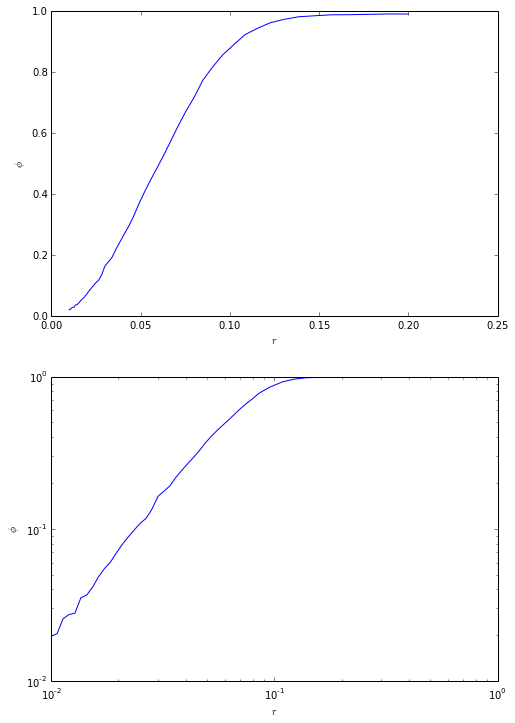
\includegraphics[width=10cm]{../img/r_phi_1.png}
        \caption{横軸$r$,縦軸$\phi = 1- (\text{クラスターの数})/(\text{点の総数})$としたグラフ}
        \label{fig:f16}
    \end{center}
\end{figure}
両対数プロットを見て分かるように,$r$の小さい領域では,ベキで近似することができそうであることが分かる。図\ref{fig:f17}には,この両対数グラフの$0<r<0.07$の範囲を直線でフィッティングしたものを示す。このときの傾きは,およそ1.86であった。
\begin{figure}[H]
    \begin{center}
        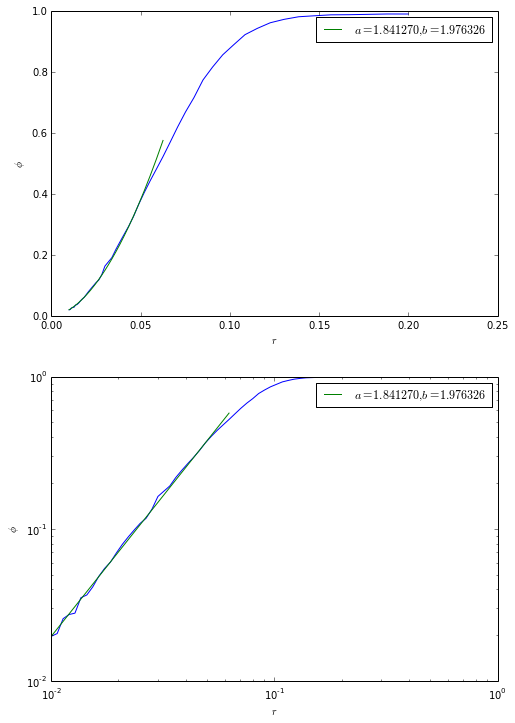
\includegraphics[width=10cm]{../img/r_phi_1_power.png}
        \caption{図\ref{fig:f16}の$0<r<0.07$の範囲をべき乗に近似したもの}
        \label{fig:f17}
    \end{center}
\end{figure}

また,これはS字型の曲線(シグモイド曲線)なので,その代表的な関数系である
\begin{eqnarray}\phi (r) = 1 - \exp \left[ -  \left( \frac{r}{\omega} \right)^{2} \right]\label{eq:e4}
\end{eqnarray}
としてパラメータ$\omega$に関して最小2乗法でフィッティングを行った。このときは先ほどの場合とは異なり,$r$の比較的大きい領域のデータを含んでいてもよい。得られたパラメータの値は$\omega=0.0715$ほどであり,図\ref{fig:f17}でべきで近似した場合に比べて,よくフィッティングできている。
\begin{figure}[H]
    \begin{center}
        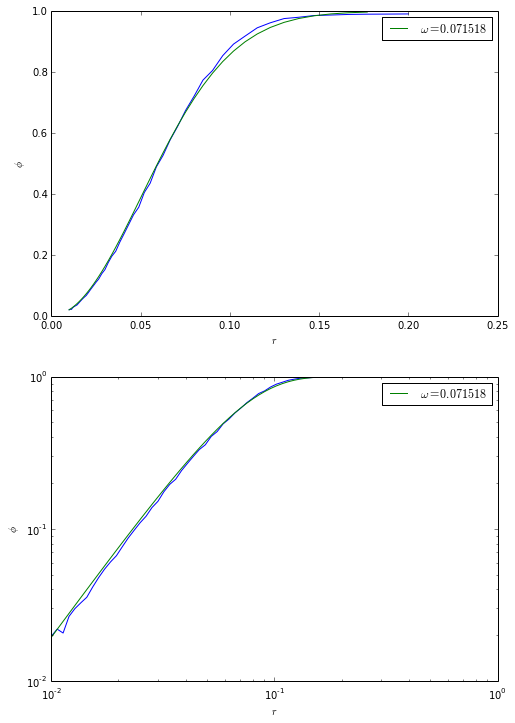
\includegraphics[width=10cm]{../img/r_phi_1_sigmoid.png}
        \caption{図\ref{fig:f16}をシグモイド曲線(\ref{eq:e4})に近似したもの}
        \label{fig:f18}
    \end{center}
\end{figure}
また,(\ref{eq:e4})式は$\phi = 1- (\text{クラスターの数})/(\text{点の総数})$の形との整合もとれているように思われる。

% =============================================================================

\subsection{モデルの説明}
このモデルでは,3.2で考えたモデルと同様に,点$x$をそれまでに選択された点からの近さで選んでゆくようなモデルを考えることにする。

これまで考えてきたモデルとの大きな相違は,点を選択していく過程をは始める前に,すべての$x$について,自分から近い位置にある点同士をエッジで結んでいき,クラスターを形成することである。こうして得られたクラスター$y$について,その一つ前に選ばれた点$x$から最も近い点を含む$y$から,次の時刻の点が選ばれるとする。このとき$y$の中から点を選ぶ方法は,そのクラスター内に含まれる点の属するそれぞれの$X$に割り当てられた重みによって決定されるとする。

このモデルの着想を得るにあたって,実際の話し合いの際に,人が多くなることによって人がどのように考えるか,ということに影響を受けている。すなわち,話し合いに参加する人が多いほど,自分の意見と同じ様な意見をもつ人がいるだろう,と思う効果であり,$X_{i}$に割り当てられた重みは,個人の発言力をあらわしていると考えることができる。

シミュレーションにおいてクラスター化を行う際には,自分と他の点との間の距離を測り,これが$r$より小さいものの間にエッジを張ることにする。このとき,(特に$r$が小さいときに)効率よく近傍点を探すことができるよう,はじめに全体を長さ$l(>r)$の正方形の領域(セル)に分割し,それぞれの点がどのセルに属しているかを記録しておく。このようにすると,近傍点を探す際には,自分の属するセルとその周囲8マスを含めた9つのセルの中にある点のみについて調べればよい。このようにしてすべての点について順番に閾値$r$の内部にある点を選択していく。このとき領域内に入ったすべての点にクラスター番号が与えられていない時には,通し番号でクラスター番号を割り当てる。閾値$r$で定められる領域内に,より小さいクラスター番号をもつ点が存在する時には,その中で一番小さいクラスター番号を,接続しているすべての点に同じクラスター番号を付与する。このようにすれば,既に存在するクラスターとの間の融合などを考慮に入れたクラスター化が行える。また,今回のシミュレーションでは,$X_{i}$の違いによる選択確率の違いはないものとした。

\subsection{シミュレーション結果}
図\ref{fig:f15}に,$r=0.07, K=20, N=4, S=20$としたときに実際にどのようにクラスターが形成され,点が選択されていくかの様子を示した図を載せる。グラフで薄いグレーで描かれた線はノード間の距離が$r$より小さいために張られたエッジであり,これが連結しているひとまとまりがクラスターである。青色の線は,選ばれた点同士をつなぐ(有向)エッジであり,振られている番号は時刻$k$に張られたエッジであることを表す。
\begin{figure}[H]
    \begin{center}
        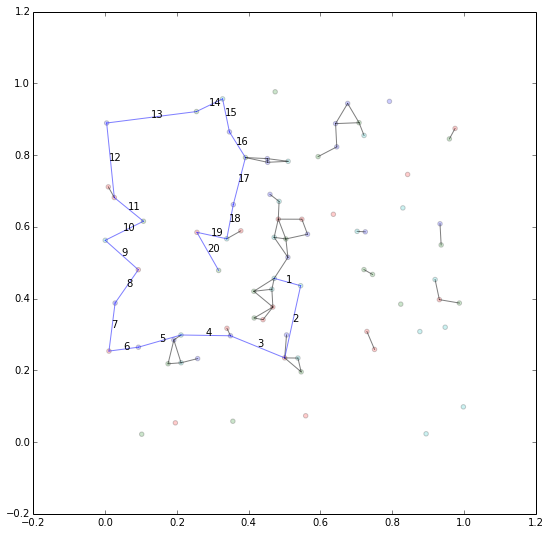
\includegraphics[width=10cm]{../img/cluster.png}
        \caption{近傍点をクラスター化するモデルのシミュレーション結果の例}
        \label{fig:f15}
    \end{center}
\end{figure}

このシミュレーションでは,考えるべき問題が二つある。一つは$r$によって作られるクラスターに関する性質である。もうひとつは,選ばれた点によって作られた軌跡に関するものだである。ただし,それぞれが独立でないために,完全に分けて考えることはできない。

まずは,閾値$r$と,点の密度に関係してクラスターがどのように形成されるかについての議論をしていくことにする。図\ref{fig:f16}は閾値$r$を変えたときの,点の総数に対するクラスターの数の関係を示している。横軸$r$,縦軸$\phi = 1- (\text{クラスターの数})/(\text{点の総数})$として,通常の軸でのプロット(上段)と両対数プロット(下段)を取っており,縦軸の値は100回の試行の平均をとったものとなっている。
\begin{figure}[H]
    \begin{center}
        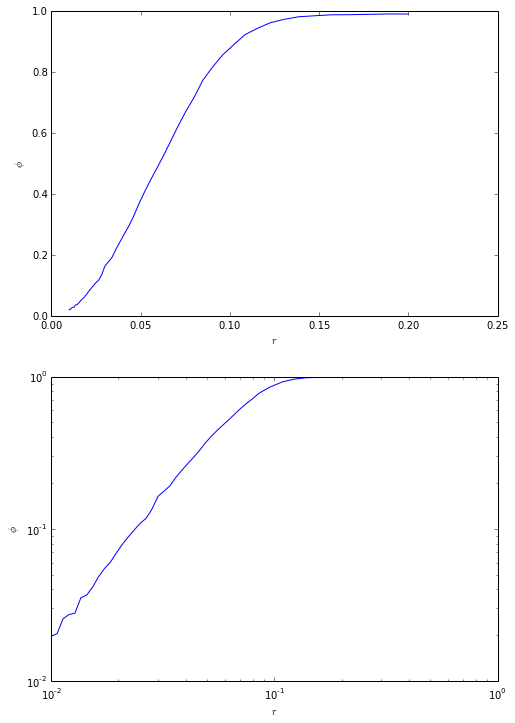
\includegraphics[width=10cm]{../img/r_phi_1.png}
        \caption{横軸$r$,縦軸$\phi = 1- (\text{クラスターの数})/(\text{点の総数})$としたグラフ}
        \label{fig:f16}
    \end{center}
\end{figure}
両対数プロットを見て分かるように,$r$の小さい領域では,ベキで近似することができそうであることが分かる。図\ref{fig:f17}には,この両対数グラフの$0<r<0.07$の範囲を直線でフィッティングしたものを示す。このときの傾きは,およそ1.86であった。
\begin{figure}[H]
    \begin{center}
        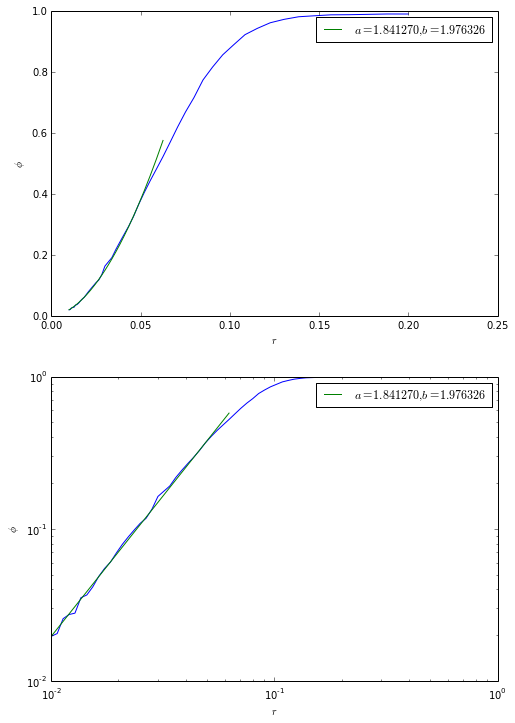
\includegraphics[width=10cm]{../img/r_phi_1_power.png}
        \caption{図\ref{fig:f16}の$0<r<0.07$の範囲をべき乗に近似したもの}
        \label{fig:f17}
    \end{center}
\end{figure}

また,これはS字型の曲線(シグモイド曲線)なので,その代表的な関数系である
\begin{eqnarray}\phi (r) = 1 - \exp \left[ -  \left( \frac{r}{\omega} \right)^{2} \right]\label{eq:e4}
\end{eqnarray}
としてパラメータ$\omega$に関して最小2乗法でフィッティングを行った。このときは先ほどの場合とは異なり,$r$の比較的大きい領域のデータを含んでいてもよい。得られたパラメータの値は$\omega=0.0715$ほどであり,図\ref{fig:f17}でべきで近似した場合に比べて,よくフィッティングできている。
\begin{figure}[H]
    \begin{center}
        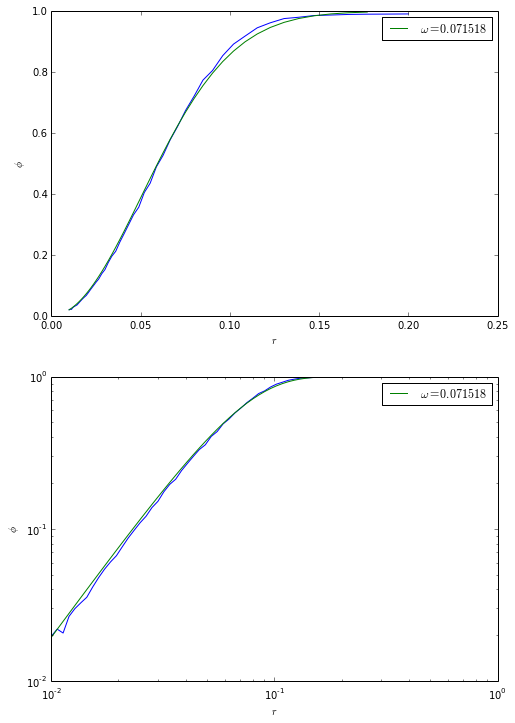
\includegraphics[width=10cm]{../img/r_phi_1_sigmoid.png}
        \caption{図\ref{fig:f16}をシグモイド曲線(\ref{eq:e4})に近似したもの}
        \label{fig:f18}
    \end{center}
\end{figure}
また,(\ref{eq:e4})式は$\phi = 1- (\text{クラスターの数})/(\text{点の総数})$の形との整合もとれているように思われる。

次に,$X_{i}$の数が変化したときにステップ間の平均移動距離$\phi$がどう変化するかについて見てみることにする。このとき,点$x$の総数$M$と$X_{i}$の数$N$,$X_{i}$あたりの点の数$S$の間には比例の関係($M=N\times S$)が成り立っており,$N$を増やすことと$S$を増やすことはこの場合等価であるから,より細かく値を刻むことのできる$S$を変化させたときのクラスター数との間の関係について調べた。横軸を$S$,縦軸を平均のステップ間距離$\phi$としたグラフを図\ref{fig:f19}に示す。このときの$N$は$N=6$であり,$r=0.07$で,100回の試行を平均したものとなっている。
\begin{figure}[H]
    \begin{center}
        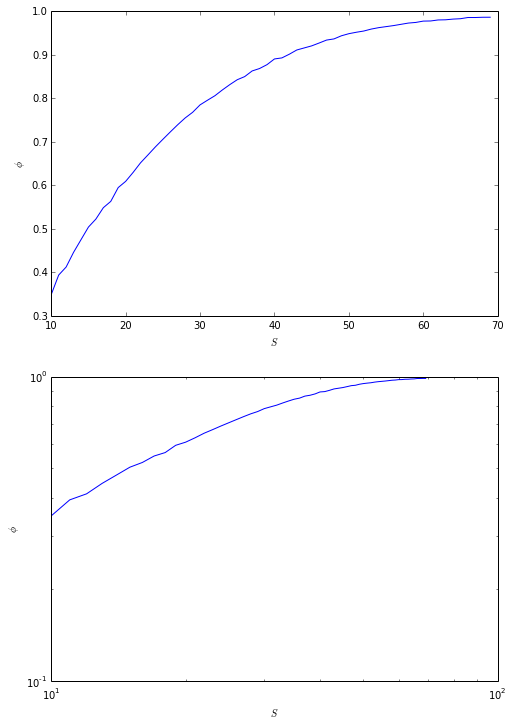
\includegraphics[width=10cm]{../img/S_phi_1.png}
        \caption{$S$を変化させたときのステップ間の平均距離}
        \label{fig:f19}
    \end{center}
\end{figure}

次に、各ステップ間の平均移動距離$l$を計算し、それが$N$によってどのように変化するかを図\ref{fig:f24}に示した。このとき$X_{i}$のもつ点の数$S=20$、クラスタ化閾値$r=0.07$とした。
\begin{figure}[H]
    \begin{center}
        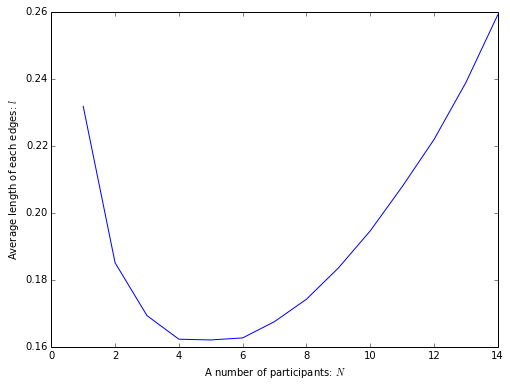
\includegraphics[width=12.5cm]{../img/N_l.png}
        \caption{ステップ間距離の平均値$l$と$N$の間の関係}
        \label{fig:f24}
    \end{center}
\end{figure}
このグラフを見て分かるように、$l$は$N$の関数として見たとき下に凸な関数となっている。このようなグラフとなるのは、先程まで考えたように$N$が増えると点の密度が大きくなり、同じ$r$でもクラスターの融合が進むので、結果的にクラスター間の距離は離れることになるということ、それから点の密度が小さいときには、クラスターは形成されにくいが、かわりに各点間の距離は広がるために各ステップ間の距離も大きくなる、と説明できる。

ここまで考えてきた各ステップ間の距離というのは、はじめに設定としてイメージしていた会議を思い浮かべると、意見間の差異を表すことになる。この値が小さいということは、選択された意見の間につながりが見られること、妥当な思考の過程によって次の意見が提出されたことを意味していると見ても良いかもしれない。逆にこの値が大きい時には、意見と意見の間の関連が小さいということを意味しており、それゆえ選択された意見間は、およそつながりがなさそうな意見になっていると言うことができる。つまり突拍子もない意見が提出されている、ということであり、生産的な会議になっているとは考えにくい。





\chapter{結論}

\bibliographystyle{junsrt}

\nocite{West04041997}
\nocite{curvature}
\nocite{allo1}
\nocite{allo2}
\nocite{allo3}
\nocite{allo4}
\nocite{allo5}
\nocite{kaigi1}
\nocite{kaigi2}
\nocite{kaigi3}
\nocite{kaigi4}
\nocite{self-organization}
\bibliography{../reference}


{\Large Appendix}


以下にはシミュレーションで用いたプログラム群(Pythonで書かれている)へのURLを記載しておく。リンクをクリックすると、WebブラウザでGithubの該当リポジトリを開くことができる。

\href{https://github.com/ssh0/sotsuron_for_public}{https://github.com/ssh0/sotsuron\_for\_public}


\newpage
\chapter*{}
\section*{謝辞}
本卒業研究にあたって、指導教員の山崎義弘先生をはじめ、同研究室の皆様には大変お世話になりました。
研究テーマの決定や、それ以降の研究の内容に関するアドバイスなどをいただいたおかげで、考察を進めることができたと思います。
重ねてここにお礼申し上げます。

\end{document}
